% Mindmap — Idéation Podcast Conso (v6 — fewer nodes, more space)
% Compile with: xelatex 02-mindmap-ideation.tex
\documentclass[border=12mm]{standalone}

\usepackage{fontspec}
\usepackage{xcolor}
\usepackage{tikz}
\usetikzlibrary{mindmap}

\setmainfont{Avenir Next}[UprightFont=* Regular, BoldFont=* Bold]
\setsansfont{Avenir Next}

\definecolor{navy}{HTML}{221C46}
\definecolor{cBlue}{HTML}{00B4F0}
\definecolor{cPink}{HTML}{FF4D6A}
\definecolor{cYellow}{HTML}{E8A020}
\definecolor{cGreen}{HTML}{1DA855}
\definecolor{cGray}{HTML}{7B8494}
\definecolor{cTon}{HTML}{3D5A99}

\begin{document}

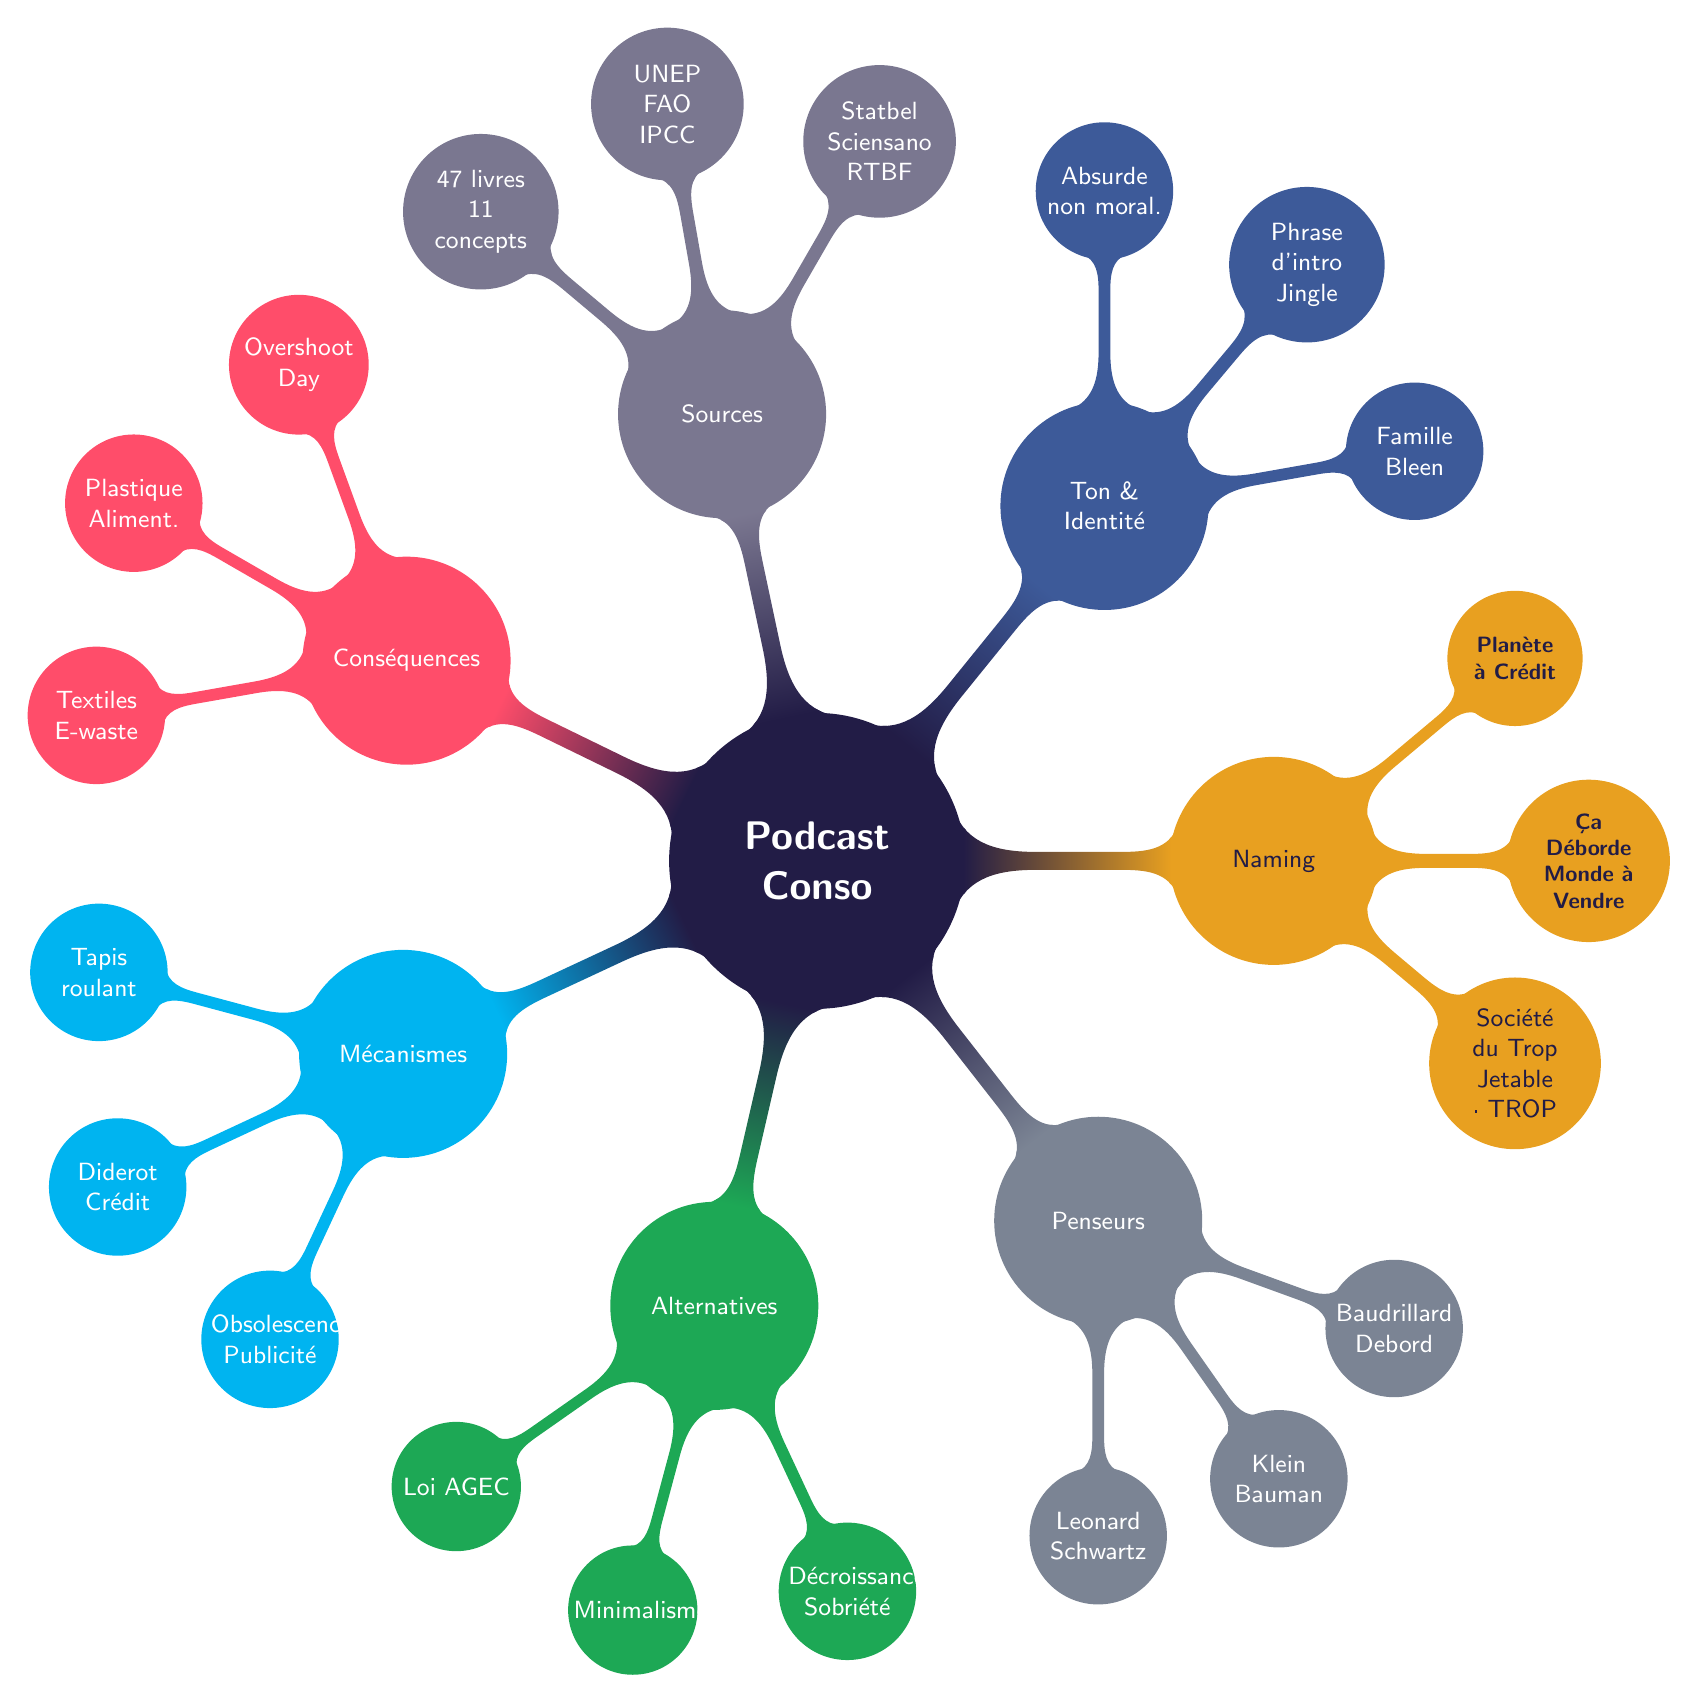
\begin{tikzpicture}[
  mindmap,
  every node/.style={concept, font=\sffamily\small, align=center},
  grow cyclic,
  concept color=navy,
  text=white,
  level 1/.append style={
    level distance=5.8cm,
    sibling angle=51.4,
    font=\sffamily\bfseries,
    minimum size=2.6cm,
  },
  level 2/.append style={
    level distance=4cm,
    sibling angle=50,
    font=\sffamily\footnotesize,
    minimum size=1.6cm,
  },
]

\node[font=\sffamily\bfseries\Large, minimum size=3.2cm] {Podcast\\Conso}
%
% ─── CONSÉQUENCES ───
  child[concept color=cPink, grow=154] {
    node {Cons\'equences}
    child[grow=190] { node {Textiles\\E-waste} }
    child[grow=150] { node {Plastique\\Aliment.} }
    child[grow=110] { node {Overshoot\\Day} }
  }
%
% ─── MÉCANISMES ───
  child[concept color=cBlue, grow=205.7] {
    node {M\'ecanismes}
    child[grow=245] { node {Obsolescence\\Publicit\'e} }
    child[grow=205] { node {Diderot\\Cr\'edit} }
    child[grow=165] { node {Tapis\\roulant} }
  }
%
% ─── ALTERNATIVES ───
  child[concept color=cGreen, grow=257.1] {
    node {Alternatives}
    child[grow=295] { node {D\'ecroissance\\Sobri\'et\'e} }
    child[grow=255] { node {Minimalisme} }
    child[grow=215] { node {Loi AGEC} }
  }
%
% ─── PENSEURS ───
  child[concept color=cGray, grow=308.6] {
    node {Penseurs}
    child[grow=340] { node {Baudrillard\\Debord} }
    child[grow=305] { node {Klein\\Bauman} }
    child[grow=270] { node {Leonard\\Schwartz} }
  }
%
% ─── NAMING ───
  child[concept color=cYellow, text=navy, grow=360] {
    node[text=navy] {Naming}
    child[grow=40] { node[font=\sffamily\footnotesize\bfseries, text=navy] {Plan\`ete\\\`a Cr\'edit} }
    child[grow=0] { node[font=\sffamily\footnotesize\bfseries, text=navy] {\c{C}a D\'eborde\\Monde \`a Vendre} }
    child[grow=-40] { node[text=navy] {Soci\'et\'e du Trop\\Jetable · TROP} }
  }
%
% ─── TON ───
  child[concept color=cTon, grow=51.4] {
    node {Ton \&\\Identit\'e}
    child[grow=90] { node {Absurde\\non moral.} }
    child[grow=50] { node {Phrase d'intro\\Jingle} }
    child[grow=10] { node {Famille\\Bleen} }
  }
%
% ─── SOURCES ───
  child[concept color=navy!60, grow=102.9] {
    node {Sources}
    child[grow=140] { node {47 livres\\11 concepts} }
    child[grow=100] { node {UNEP FAO\\IPCC} }
    child[grow=60] { node {Statbel\\Sciensano\\RTBF} }
  }
;

\end{tikzpicture}

\end{document}
